\section{Experimental Data}
\label{sec:data}


    We generated several problem suites with \fuzzer{} that made one solver perform poorly, but not others. These suites are \theSuites{}. Figure~\ref{fig:cvc-hard} shows the suites that were uniquely difficult for \cvc{}. Figure~\ref{fig:z3str3-hard} shows the suites that were uniquely difficult for \us{}. All experiments were run in series on the same Linux computer, with a timeout of 15 seconds. \todo{Specify CPU, memory}

    \begin{figure}[h]
        \vspace{-0.2in}
        \begin{subfigure}{.5\textwidth}
            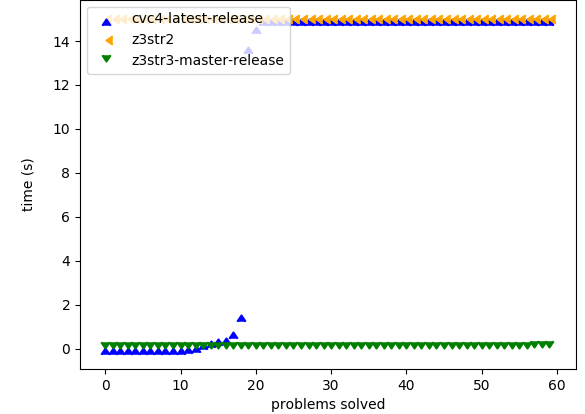
\includegraphics[width=\textwidth]{data/graphs/concats-extracts-small.png}                   
            \vspace{-0.25in}
            \caption{Performance on concats-extracts-small} 
            \label{fig:concats-extracts-small}
        \end{subfigure}
        \begin{subfigure}{.5\textwidth}
            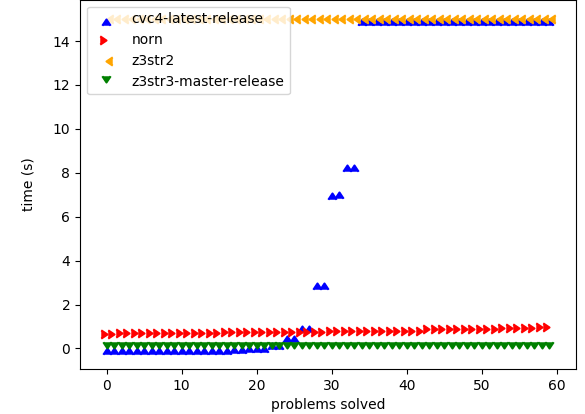
\includegraphics[width=\textwidth]{data/graphs/different-prefix.png}            
            \vspace{-0.25in}
            \caption{Performance on different-prefix}
            \label{fig:different-prefix}
        \end{subfigure}
        \vspace{-0.1in}
        \caption{Problems hard for \cvc{}}
        \label{fig:cvc-hard}
        \vspace{-0.3in}
    \end{figure}

    \begin{figure}[h]
    \vspace{-0.25in}
        \begin{subfigure}{.5\textwidth}
            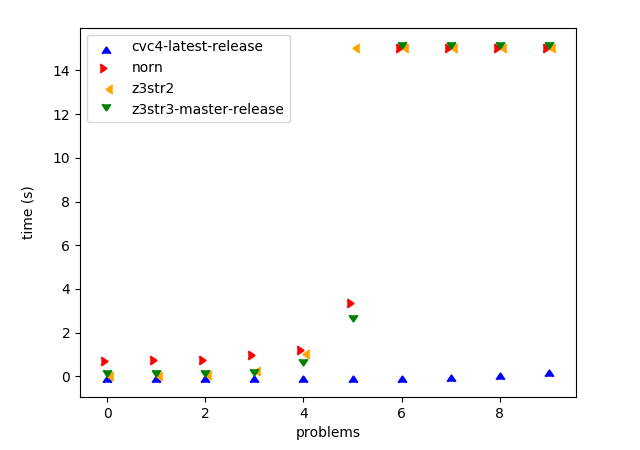
\includegraphics[width=\textwidth]{data/graphs/concats-balanced.png}
            \label{fig:concats-balanced}
            \vspace{-0.25in}
            \caption{Performance on concats-balanced}
        \end{subfigure}
        \begin{subfigure}{.5\textwidth}
            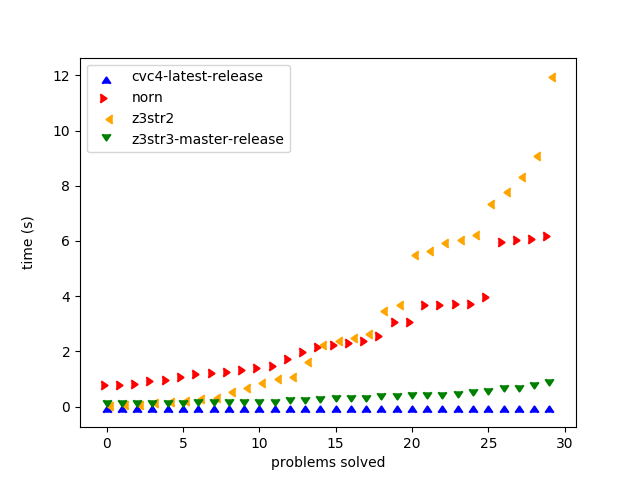
\includegraphics[width=\textwidth]{data/graphs/concats-small.png}
            \label{fig:concats-small}
            \vspace{-0.25in}
            \caption{Performance on concats-small}
        \end{subfigure}
        \vspace{-0.1in}
        \caption{Problems hard for \us{}}
        \label{fig:z3str3-hard}
        \vspace{-0.3in}
    \end{figure}

    
\section{Usefulness to \us{}: A Case Study}
\label{sec:analysis}

        In this section we describe a number of performance-related issues and opportunities for new heuristics
        which were exposed in \us{} by \fuzzer{} to illustrate the utility and value of the tool in solver development.
        
        
\subsection{Defects discovered and fixed in \us{}}


The first issue we found caused \us{} to perform poorly when equivalence classes 
of arithmetic terms were very large (e.g. the lengths of many strings were equal
to 0). This issue was detected by the \texttt{Concats} problem suite. The slowdown 
was caused by a loop over terms in the same equivalence class to search for an 
integer constant. The fix was to check the root of the equivalence class for the 
integer constant, as Z3 makes ``interpreted terms'' (e.g. constants) the root of 
equivalence classes whenever possible. This issue was last observed in commit 
\texttt{6308636}, and was fixed in commit \texttt{3865c45}.


The second issue, which was exposed by the \texttt{Lengths} suite, caused \us{} to 
perform poorly when a variable has a large length constraint.
The slowdown was caused by the solver performing a search for a satisfying length
even when the input formula explicitly constrained the exact length of a string term.
The fix was to check whether the integer solver had already assigned a length value
before searching for length, and skip the search if this was the case.
This issue was last observed in commit \texttt{66bc68f}, and was fixed in commit 
\texttt{7b536e9}.    
%The slowdown was  caused by the solver performing a linear search for a satisfying length when 
%producing a model for the variable. This issue was an inconsistency between the 
%implementation and the behavior described in the \us{} paper \cite{z3str3}. 
%This issue was last observed in commit \texttt{66bc68f}, and was fixed in commit 
%\texttt{7b536e9}.    
    
    

\subsection{Solving heuristics}


In order to improve the efficiency of any solver, discovering new heuristics is crucial.
As an illustrative example, consider detection of conflicting constraints.
A solver that follows the string constraint solving algorithm and gradually propagates
the (dis)equalities discovered along the way will eventually detect a conflict.
However, in many scenarios, a conflict can be discovered ``early'' before trying to
figure out the relationships among subterms and propagating the facts.
The benefits of this eager approach are clear: this saves the effort of reasoning about
subterms and propagating observations, as a conflict will eventually be reached in either case,
forcing conflict analysis and a backjump.
As reported in existing works, heuristics of this form usually lead to significant improvements.
However, the process of discovering such heuristics is extremely challenging,
as they are usually learned from a class of examples whose commonalities
are not always obvious or immediately indicative of such inefficiencies.

The instances in the \texttt{concats-big} suite generated by \fuzzer{} helped us 
discover a missing heuristic in \us{}. In particular, \us{} didn't make full use 
of the solving context (e.g. some terms are empty strings) to simplify the 
concatenations of a long list of string terms before trying to reason about the 
equivalences among subterms. \us{} therefore introduced a large number of unnecessary
intermediate variables and propagations.
As an immediate consequence of the \texttt{concats-big} benchmarks, we were able to identify
the factors common to these instances and rapidly formulate a hypothesis as to why they were
performing poorly. This allowed us to move forward with the development of new heuristics
to resolve these issues and achieve better performance.


% In this section, we analyse our experimental results. We discuss the causes of 
% \us{}'s poor performance on the two problem suites: \textit{concats-balanced} 
% and \textit{concats-big}. We were not equipped well enough to debug the 
% behaviours of the other solvers, but we provide our data in hopes that they will 
% be useful to the solvers' authors.

%     \subsection{\us{} on concats-balanced}
%         \todo{Dmitry with help: Explain why \us{} performs poorly on this suite.}

        
        
        
% X = "solution"
% X = (((A.B).(C.D)).((E.F).(G.H))).
%     (((I.J).(K.L)).((M.N).(O.P)))

    % \subsection{\us{} on concats-big}

    %     \todo{Dmitry with help: Explain why \us{} performs poorly on this suite.}

% X = "solution"
% X = (A.(B.(C.(D.(E.(F.(G.H)))))))
